\documentclass{article}
%\usepackage{graphicx} 
%\usepackage[
  paperheight=8.5in,
  paperwidth=5.5in,
  left=10mm,
  right=10mm,
  top=20mm,
  bottom=20mm]{geometry}
\usepackage[utf8]{inputenc}

%%\usepackage{biblatex}
\usepackage{graphicx}
\usepackage{wrapfig}
\usepackage[bottom]{footmisc}
\usepackage{listings}
\usepackage{enumitem}

\usepackage{wrapfig}
\usepackage{ragged2e}

\usepackage{array}
\usepackage[table]{xcolor}
\usepackage{multirow}
\usepackage{booktabs}
\usepackage{hhline}
\definecolor{palegreen}{rgb}{0.6,0.98,0.6}

\usepackage{amsmath}
\usepackage{amssymb}
\usepackage{multicol}
\usepackage{lipsum}
\usepackage{hyphenat}
\PassOptionsToPackage{hyphens}{url}
\usepackage{url}

\usepackage{rotating}

\usepackage{pdfpages}

%% support use of straight quotes in code listings
\usepackage[T1]{fontenc}
\usepackage{textcomp}
\usepackage{listings}
\lstset{upquote=true}

%% for shrinking space between lines
\usepackage{setspace}

\usepackage{caption}

\newcommand*{\affaddr}[1]{#1} % No op here. Customize it for different styles.
\newcommand*{\affmark}[1][*]{\textsuperscript{#1}}
\newcommand*{\email}[1]{\small{\texttt{#1}}}
\newcommand{\tarot}{\textsc{Tarot}}
\renewcommand*\contentsname{\centering Table of Contents}

\renewcommand{\footnoterule}{%
  \kern -3pt
  \hrule width \textwidth height 0.5pt
  \kern 2pt
}

\usepackage{titlesec}
\titleformat*{\section}{\large\bfseries}
\titleformat*{\subsection}{\normalize\bfseries}
\titleformat*{\subsubsection}{\normalize\bfseries}

% define variables
\newcommand{\confOrdinal}{34th}
\newcommand{\confName}{South Central}
\newcommand{\confDates}{March 31st}
\newcommand{\confYear}{2023}
\newcommand{\confSchool}{Stephen F. Austin State University}
\newcommand{\confCity}{Nacogdoches, TX}
\newcommand{\journalVolume}{38}
\newcommand{\journalNumber}{7}
\newcommand{\journalMonth}{April}
\newcommand{\journalYear}{2023}
\newcommand{\regionalEditor}{Mustafa Al-Lail}
\newcommand{\regionalEditorSchool}{Texas A\&M International University}


%\addbibresource{1048.bib}

% Note to editor: The example formatting guide marked citations with simple square brackets, without superscripts such as [1]. In this paper, several educational examples are used which heavily involve array notation, which also uses square brackets without superscripts. This could possibly confuse readers as to what is a citation versus an example value, so citations have been placed in superscript.

\title{Comparative Sequential and Parallel Discrete Signal Convolution Algorithms: A Case Study\footnote{\protectCopyright \copyright \confYear\ by the Consortium for Computing Sciences in Colleges.
Permission to copy without fee all or part of this material is granted provided
that the copies are not made or distributed for direct commercial advantage,
the CCSC copyright notice and the title of the publication and its date appear,
and notice is given that copying is by permission of the Consortium for
Computing Sciences in Colleges.  To copy otherwise, or to republish, requires
a fee and/or specific permission.
}
}
\author{
Caleb Sneath and Eduardo Colmenares\\
Computer Science\\
Midwestern State University\\
\email{\{caleb.sneath, eduardo.colmenares\}@msutexas.edu}\\
}
\begin{document}
\maketitle

\begin{abstract}
Case studies play an important role in the testing and verification of prevailing conventional wisdom, the collection of knowledge in a new and quick format, and to potentially answer several minor questions at once which on their own are not worthy of deeper inquiry. Case studies ideally should have a clear focus, provide at least one good question which can be answered by the case study, and ensure that their creation provides some tangible educational benefit to one or more fields. This paper focuses on discrete signal convolution problems, as well as multiple algorithms which can be used to solve them, particularly from the viewpoint of output signal analysis. 

The discrete one-dimensional (1D) signal convolution problem has applications in statistics, physics, music, machine learning, and electrical engineering. This paper aims to answer how much a parallel GPU-based approach might speed up the problem as well as ways an existing library implementation can differ from a simpler parallel algorithm implementation from scratch. This paper presents a case study that makes extensive use of GPU programming and should benefit not only those involved in computer science, but also those involved in any mathematics, engineering, or fields of science in which signal convolution is a concern. 
\end{abstract}

\section{Methodology}
This paper explores 1D convolution by breaking its discussion into six parts. The first part aims to provide a quick definition and summary of the relevant background information for convolution. The second step goes over one possible method to solve 1D convolution problems by hand. This section also contains an illustrative example. The third part discusses ways in which the 1D convolution problem can be programmed. This section describes two methods to view 1D convolution problems that help break it down easier into sequential code, a section on how to modify one of the sequential algorithms to instead take advantage of GPU parallelization, and a section which briefly mentions some modifications which a more complicated library might use in order to further optimize the problem. The sections on sequential and parallel code each include example C++/CUDA implementations of 1D convolution algorithms. Finally, the last part of this paper summarizes an experiment to time one of the sequential approaches as well as the parallel GPU approach mentioned in in part three of this paper. This section includes tables of the results of the average execution times and speedups across different problem sizes. The averages for each input size were obtained from 35 trials each of input matrix sizes in increasing powers of two. For each trial, the filter size remained constant with a size of four, and each item of the output matrix was computed by a single GPU thread each for the parallel trials. This section also briefly lists the hardware specifications of the test machine used, although all trials were conducted on the same computing cluster.

\section{Problem Description}
Convolution is an operation like addition or subtraction, but for matrices rather than individual numbers. It is represented by the ``*'' symbol, meaning that for matrices it is important to properly distinguish between multiplication and convolution. For this reason, normal multiplication should be represented by ``x'', and the dot product by a single dot. As an operation, convolution is commutative so the order of the two matrices to be convolved does not matter \affmark[{\cite{smith}\cite{KIRANYAZ2021107398}}]. The larger matrix is often referred to as the input matrix or mathematically as x[n]. The smaller matrix on the other hand has a variety of commonly used terms to refer to it such as filter, kernel, convolution kernel, the point spread function, or mathematically as h[n] \affmark[\cite{smith}]. 

Standard conventions on the format of the two signal matrices to be convolved exist which make communicating and calculating 1D convolution easier. One of the matrices to be convolved should be the impulse response for a given delta function. The delta function, denoted by $\delta$[n], is a way to represent any signal in a normalized format by giving sample number zero the value of one, and all other signals a value of zero. The impulse response then is the resulting exiting symbol for the delta function] \affmark[{\cite{smith}\cite{KIRANYAZ2021107398}}]. In simple terms, the 1D convolution is a sum of products in a sliding window. For two 1D matrices, matrix h and matrix x, the convolution is formally defined by the following equation:  

\hfil $y[i]=\sum_{(j=0)}^{(M-1)} h[j]x[i-j]$ \par
\hfil Equation 1. \par

\section{The Do It by Hand Phase}
Signal convolution can be solved fairly simply by hand, although the time required to do so can be immense as the problem size expands past just a few values for the input and filter. For simplicity, this section will refer to the signal with more samples as the input signal, and the smaller signal as the filter.  This should not pose a problem in practice as convolution’s commutative property means that the order of the two signals can be freely rearranged without affecting the output \affmark[{\cite{smith}}].

One helpful method is to start by finding the total number of outputs for the output signal. This will simply be the sum of the number of elements in the input and filter signal minus one. Then, create a table with as many columns as the number of outputs in the output signal, and as many rows as the number of inputs. In the first row, starting in the first column and going right a column one number at a time, write each element of the filter, stopping when the filter is out of elements. Then, next to each of the newly added numbers, write a multiplication sign, and put the first element of the input next to each of these numbers. Next, move onto the next row. Once again, start by writing out all elements of the filter, however begin doing so one column to the right of the previous row. Next, once again place the multiplication sign next to each element, and this time add element two of the input signal. Repeat this process until there are no more rows. Next, compute the product for each cell. Finally, sum up every element within the same column, and left to right each sum is that element of the output signal.

For illustrative purposes let’s assume signal S1 is the input signal, signal S2 is the filter signal, and signal S3 is the output signal. Although this example uses signals of size 5 and 3, it is important to remember that by following the same process, any size of inputs can be solved in a similar fashion. If S1 = {1, 2, 3, 4, 5}; S2 = {5, 6, 7}; the objective is then to compute S3 = S1 * S2.

\begin{figure}[htp]
    \centering
    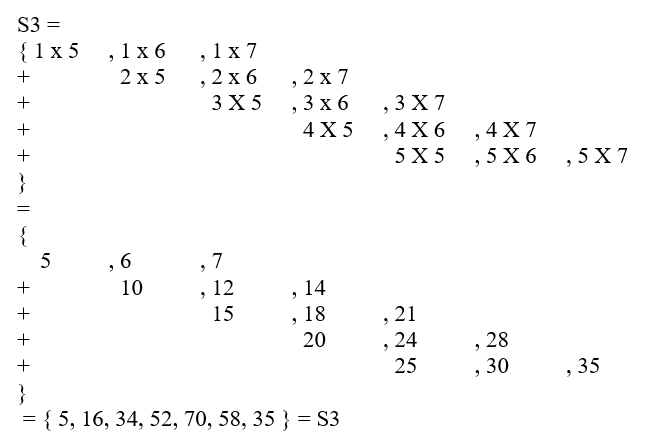
\includegraphics[width=0.85\textwidth]{1048_1.png}
    \caption{By Hand Example}
    \label{fig:hand}
\end{figure}

\section{Computational Solutions}
There are at least two different broad approaches to creating an algorithm that can solve signal convolution problems. The first broad viewpoint involves examining and therefore iterating through each input signal to determine how it contributes to each output. This is arguably better suited to a sequential approach than a parallel one as each iteration of the outer loop contributes to multiple output signals, resulting in some dependencies on multiple iterations for each output. The second viewpoint involves examining and therefore iterating across each output signal and determining how it was affected by different inputs. This algorithm is well suited to parallelization as each iteration of the outer loop can be turned into a separate thread since each element of the output can be calculated entirely independent of the others, although it is also fine for serial approaches.

\subsection{First Sequential Implementation}
The input viewpoint serial code is described by Smith\affmark[\cite{smith}] as a very intuitive algorithm to understand. Simply put, after zeroing the output signal’s array there is an outer loop which iterates from the starting element to the ending element of the input signal’s array. Then, there is an inner loop which iterates from the starting element to the ending element of the filter signal. Inside the nested loop, the output signal with an index equal to both loop counters is assigned the value of itself plus (the current input element times the current filter element). Figure 2 provides an idea of its C++ implementation.

\begin{figure}[htp]
    \centering
    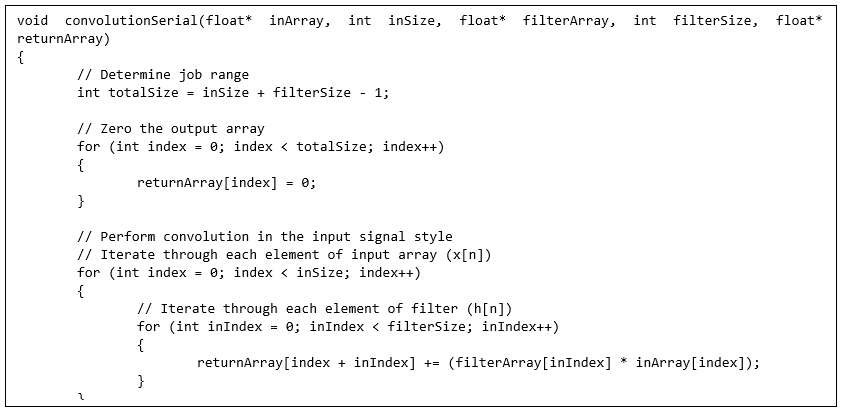
\includegraphics[width=\textwidth]{1048_2.png}
    \caption{Input Viewpoint Sequential Code}
    \label{fig:inpoint view code}
\end{figure}

\subsection{Second Sequential Implementation}
The output viewpoint is mainly more difficult to understand due to the complexity at first glance of determining which indices of the input and filter arrays correspond to which output without directly iterating through each to find out. It begins with an outer loop which iterates across each element of the output matrix. At the start of each iteration of the loop, the current output being calculated is assigned a starting value of zero. Then, an inner loop begins which iterates through each element of the filter signal array. Inside this loop, some bounds checking is done to ensure the input and filters don’t go out of bounds for their index. If they won’t, an extra step must be taken. A temporary value will be computed using the product of one point of the input and filter matrix. The filter value’s index can be obtained from the innermost loop. The input matrix item for this will be the item with the index of the current output value minus the index of the current filter value. Afterwards, this temporary value is added to the current output value. An example of the use of this temporary value is below.

\hfil Input Matrix = \{0, 2, 4, 6, 5\}	Filter Matrix = \{1, 2, 3, 5\} \par

To calculate the temporary value for the output matrix on index 3 for the innerloop value of 1, first the filter value must be obtained. The filter matrix index is obtained directly from the innerloop index, which is 1. Filter Matrix [0] is 1. Next, the input matrix value must be obtained. The input matrix index is obtained from subtracting the current output value index, 3, from the current filter value index we just obtained, 0, for an index of 3. Input Matrix [3] is 6. Calculating the product of the input and filter gives a temporary value of (6 * 1 = 6). This temporary value can then be added to the current output value, Output Matrix [3]. Figure 3 provides an idea of its C++ implementation.

\begin{figure}[htp]
    \centering
    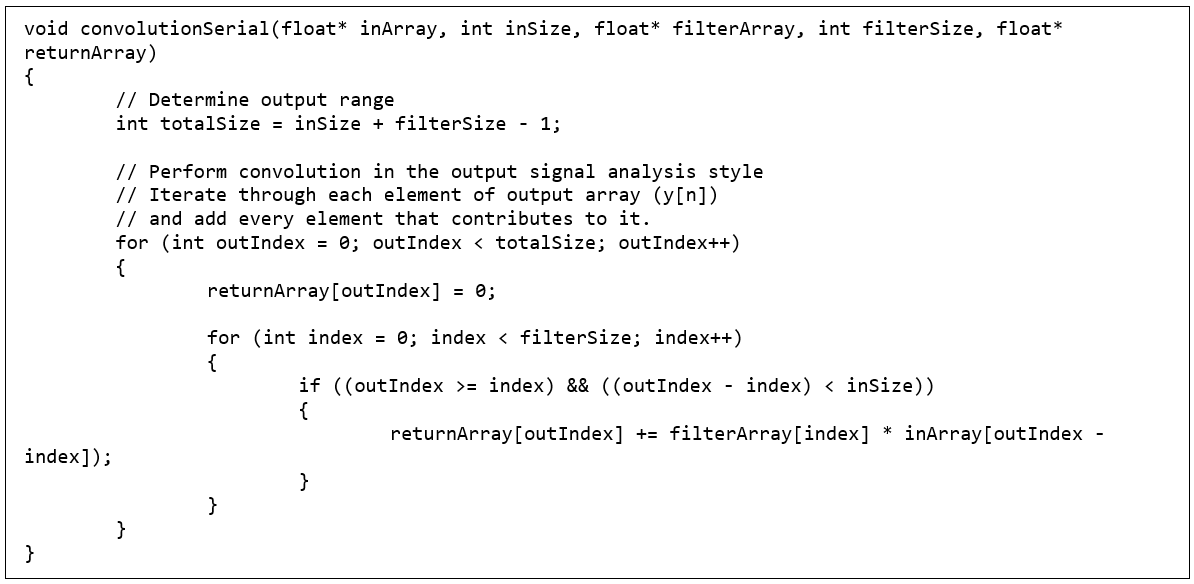
\includegraphics[width=\textwidth]{1048_3.png}
    \caption{Output Viewpoint Sequential Code}
    \label{fig:outpoint view code}
\end{figure}

\subsection{Parallel Implementation}
This paper’s illustrative parallel approach was similar to the serial output viewpoint centered algorithm with several minor adjustments. Each thread is mostly concerned with calculating one output value, however each thread may need to calculate more if it is assigned more outputs than the number of threads called, or less, meaning zero, in cases where the number of outputs isn’t evenly divisible by the number of threads per block. To meet these goals, the function begins like the sequential output viewpoint version by calculating the number of total threads as well as which job id this block and thread would translate into. Then, the outer loop is tweaked to begin only at this thread’s job id as the output index, and go up by the total number of threads each time until it is at least as large as the total number of outputs. 

Figure 4 provides an idea of its C++ implementation.

\begin{figure}[htp]
    \centering
    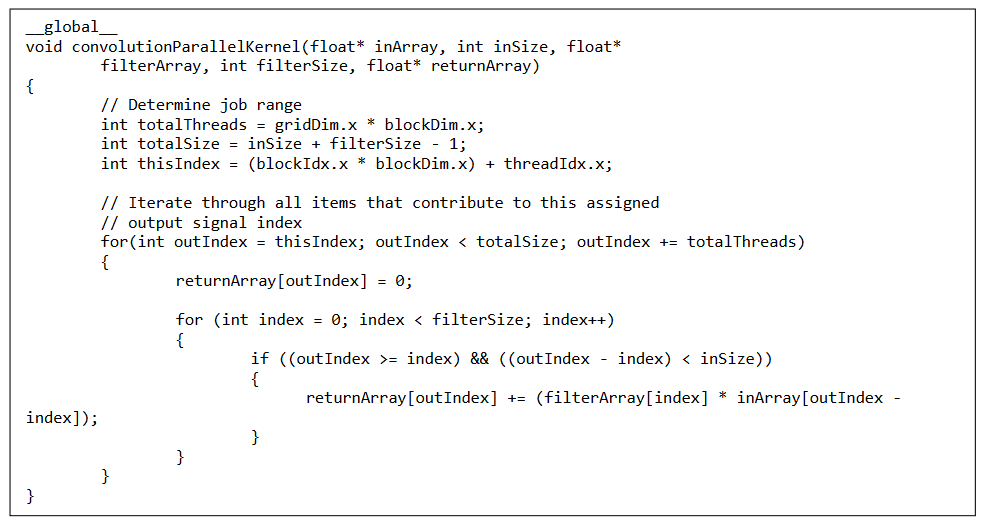
\includegraphics[width=\textwidth]{1048_4.png}
    \caption{Parallel CUDA GPU Code}
    \label{fig:parallel code}
\end{figure}

\section{Testing Environment}
All trials were performed in the same program execution on the Maverick2 computing cluster. The specifications of the Maverick2 cluster as presented by TACC are as follows \affmark[{\cite{maverick2}\cite{stampede2}\cite{geforce}}].

\begin{table}[ht]
\centering
\caption{Maverick 2 GTX Compute Node Specifications} % title of Table
\label{table:nonlin} % is used to refer this table in the text
%\begin{tabular}{ |p{3cm}|p{1.5cm}|p{0cm}|p{2.25cm}|p{1.25cm}|  }
\begin{tabular}{ |p{0.25\textwidth}|p{0.12\textwidth}|p{0.01\textwidth}|p{0.25\textwidth}|p{0.12\textwidth}|} 
 \hline
 \multicolumn{2}{|c|}{\textbf{CPU}} &  & \multicolumn{2}{|c|}{\textbf{GPU}}\\
 \multicolumn{2}{|c|}{\footnotesize\textbf{(Intel(R) Xeon(R) CPU E5-2620 v4)}} &  & \multicolumn{2}{|c|}{\textbf{(GTX 1080-TI)}}\\
 \hline
 {Processors per node:} & {2} &  & {CUDA Cores} & {3584}\\
 \hline
 {Cores per processor:} & {8} &  & {Graphics Clock (MHz)} & {1480}\\
 \hline
 {Cores per node:} & {16} &  & {Processor Clock (MHz)} & {1582}\\
 \hline
 {HW threads per core:} & {2} &  & {Graphics Performance} & {High-200,000}\\
 \hline
 {HW threads per node:} & {32} &  & \multicolumn{2}{|c|}{\textbf{Memory Specs}}\\
 \hline
 {Clock rate:} & {2.10 GHz} &  & {Standard Memory Configuration} & {11 GB GDDR5X}\\
 \hline
 {RAM:} & {128 GB} &  & {Memory Interface Width} & {352-bit}\\
 \hline
 {L1/L2/L3 Cache:} & {512KiB/ 2MiB/ 20MiB} &  & {Bandwidth (GB/Sec)} & {11 Gbps}\\
 \hline
 {Local Storage:} & {150.0 GB (~60 GB free)} &  & \multicolumn{2}{|c|}{\textbf{Thermal and Power Specs}}\\
 \hline
 {GPUs:} & {4xNVidia 1080-TI GPUs} &  & {Max. Graphics Card Power (W)} & {250}\\
 \hline
\end{tabular}
\end{table}

\section{Comparisons}
Testing revealed several predictable as well as unexpected results. As is somewhat expected, serial time grew roughly linearly for the serial approach with respect to input size. In contrast, the parallel approach started off performing weaker, but scaled significantly better as the problem size increased in comparison, with the graph showing somewhere from constant to logarithmic performance. This results in the serial program being more efficient for smaller problem sizes, but the parallel approach gaining an advantage as the problem size increases, suggesting that it may have a better algorithmic complexity.  Allocating variables, copying variables, launching multiple threads, and then recopying and freeing extra variables can constitute a relatively expensive process, so it isn’t unreasonable that for small enough problem sizes, this extra overhead is simply not a worthwhile cost to solve the problem better. 

\begin{table}[ht]
\centering
\caption{Execution Times and Speedup} % title of Table
\label{table:nonlin} % is used to refer this table in the text
%\begin{tabular}{ |p{1.5cm}|p{1.75cm}|p{1.2cm}|p{1.0cm}|p{1.2cm}|p{1.2cm}|  }
\begin{tabular}{|p{0.1\textwidth}|p{0.1\textwidth}|p{0.11\textwidth}|p{0.1\textwidth}|p{0.1\textwidth}|p{0.11\textwidth}|} 
 \hline
 \multicolumn{2}{|c|}{\small\textbf{Problem Size for Serial}} & \multicolumn{2}{|c|}{\small\textbf{Program Execution}} & \multicolumn{2}{|c|}{\small\textbf{Speedup}}\\
 \multicolumn{2}{|c|}{\small\textbf{and Parallel - GPU}} & \multicolumn{2}{|c|}{\small\textbf{Time}} & \multicolumn{2}{|c|}{\small\textbf{Relative To}}\\
 \multicolumn{2}{|c|}{\small\textbf{Threads for Parallel Only}} & \multicolumn{2}{|c|}{\small\textbf{(Seconds)}} & \multicolumn{2}{|c|}{\small\textbf{Serial}}\\
 \hline
 {\small\textbf{Size}} & {\small\textbf{GPU Threads}} & {\small\textbf{Serial}} & {\small\textbf{Parallel}} & {\small\textbf{Serial}} & {\small\textbf{Parallel}}\\

 \hline
 {1,024} & {1,027} & {0.000018} & {0.000293} & {1} & {0.061}\\
 \hline
 {2,048} & {2,051} & {0.000037} & {0.000294} & {1} & {0.126}\\
 \hline
 {4,096} & {4,099} & {0.000073} & {0.000335} & {1} & {0.218}\\
 \hline
 {8,192} & {8,195} & {0.000145} & {0.000290} & {1} & {0.500}\\
 \hline
 {16,384} & {16,387} & {0.000291} & {0.000312} & {1} & {0.933}\\
 \hline
 {32,768} & {32,771} & {0.000581} & {0.000422} & {1} & {1.377}\\
 \hline
 {65,536} & {65,539} & {0.001162} & {0.000533} & {1} & {2.180}\\
 \hline
\end{tabular}
\end{table}

One trend which warrants further investigation is the difference in how required time changes between the smaller and the larger parallel GPU based approaches. While the small input size figures produce similar averages seemingly constant and within the normal range of variance, larger input sizes begin to scale to some degree with input sizes. This doesn’t appear to be a mere outlier of the data, as similar figures were obtained across several 35-trial average runs of the program. As no thread or output should be reliant upon the work of another thread, it is possible that what is happening is that at some point, the threads simply start competing for placing required values in limited memory space. If this is indeed the case, it might be worthwhile to examine whether for a large enough problem size, factors like competition for limited memory begins to lower the relative advantage that parallel GPU approaches possess vs serial CPU approaches, or even if some modifications to use some degree of synchronization and shared memory management may allow continued increasing of performance.                                                                             
\section{Conclusions}
The average of the trials suggests that a parallel GPU based approach can but won’t always speed up signal convolution. This may be because the highly independent nature of computing each output matrix value means that the process can potentially benefit highly from the more cores that can be utilized for a larger problem. In contrast, for smaller problems it seems to be the case that the overhead required both to launch the threads, as well as in some cases the additional CUDA overhead to simply first launch a CUDA function at program start combine to make a traditional serial CPU based approach not only suitable but faster to solve these kinds of problems compared to just a fairly straightforward parallel implementation of 1D convolution. Existing libraries exist which employ more advanced techniques to increase performance even further. One potential area worth examining would be whether it is the case that these techniques also only extend to improving performance to scale better for larger datasets at the cost of creating further overhead that keeps performance behind a traditional sequential CPU-based approaches.

\medskip
\bibliographystyle{plain}
\bibliography{1048}
%\nocite{*}
%\printbibliography

\end{document}